\section{Radio Frequency Interference Analysis}

\subsection{Definition of RFI}
Radio frequency interference (RFI) consists of radio waves emitted from any Earthly source that can overcome or be confused with the target signal. Examples of RFI can include satellites, electronic equipment, and local broadband communications. Unlike statistical noise, RFI cannot be removed through smoothing or time averaging because RFI is a distinct signal and not a random variable. Instead, it must be identified and removed.\\

A roof mounted receiver located at the DRAO site called the `RFI monitor' records radio signals from all directions, providing an estimate of the expected RFI which CHORD will receive. However the RFI monitor differs in two important ways from CHORD:
\begin{itemize}
    \item CHORD is orders of magnitude more sensitive than the RFI monitor, signals that are not detectable by the RFI monitor may nonetheless impede CHORD.
    \item CHORD has a directional beam (towards the sky) while the RFI monitor is a single antenna without a dish, RFI signals travelling horizontally will be 
\end{itemize}

\begin{figure}[t]
    \centering
    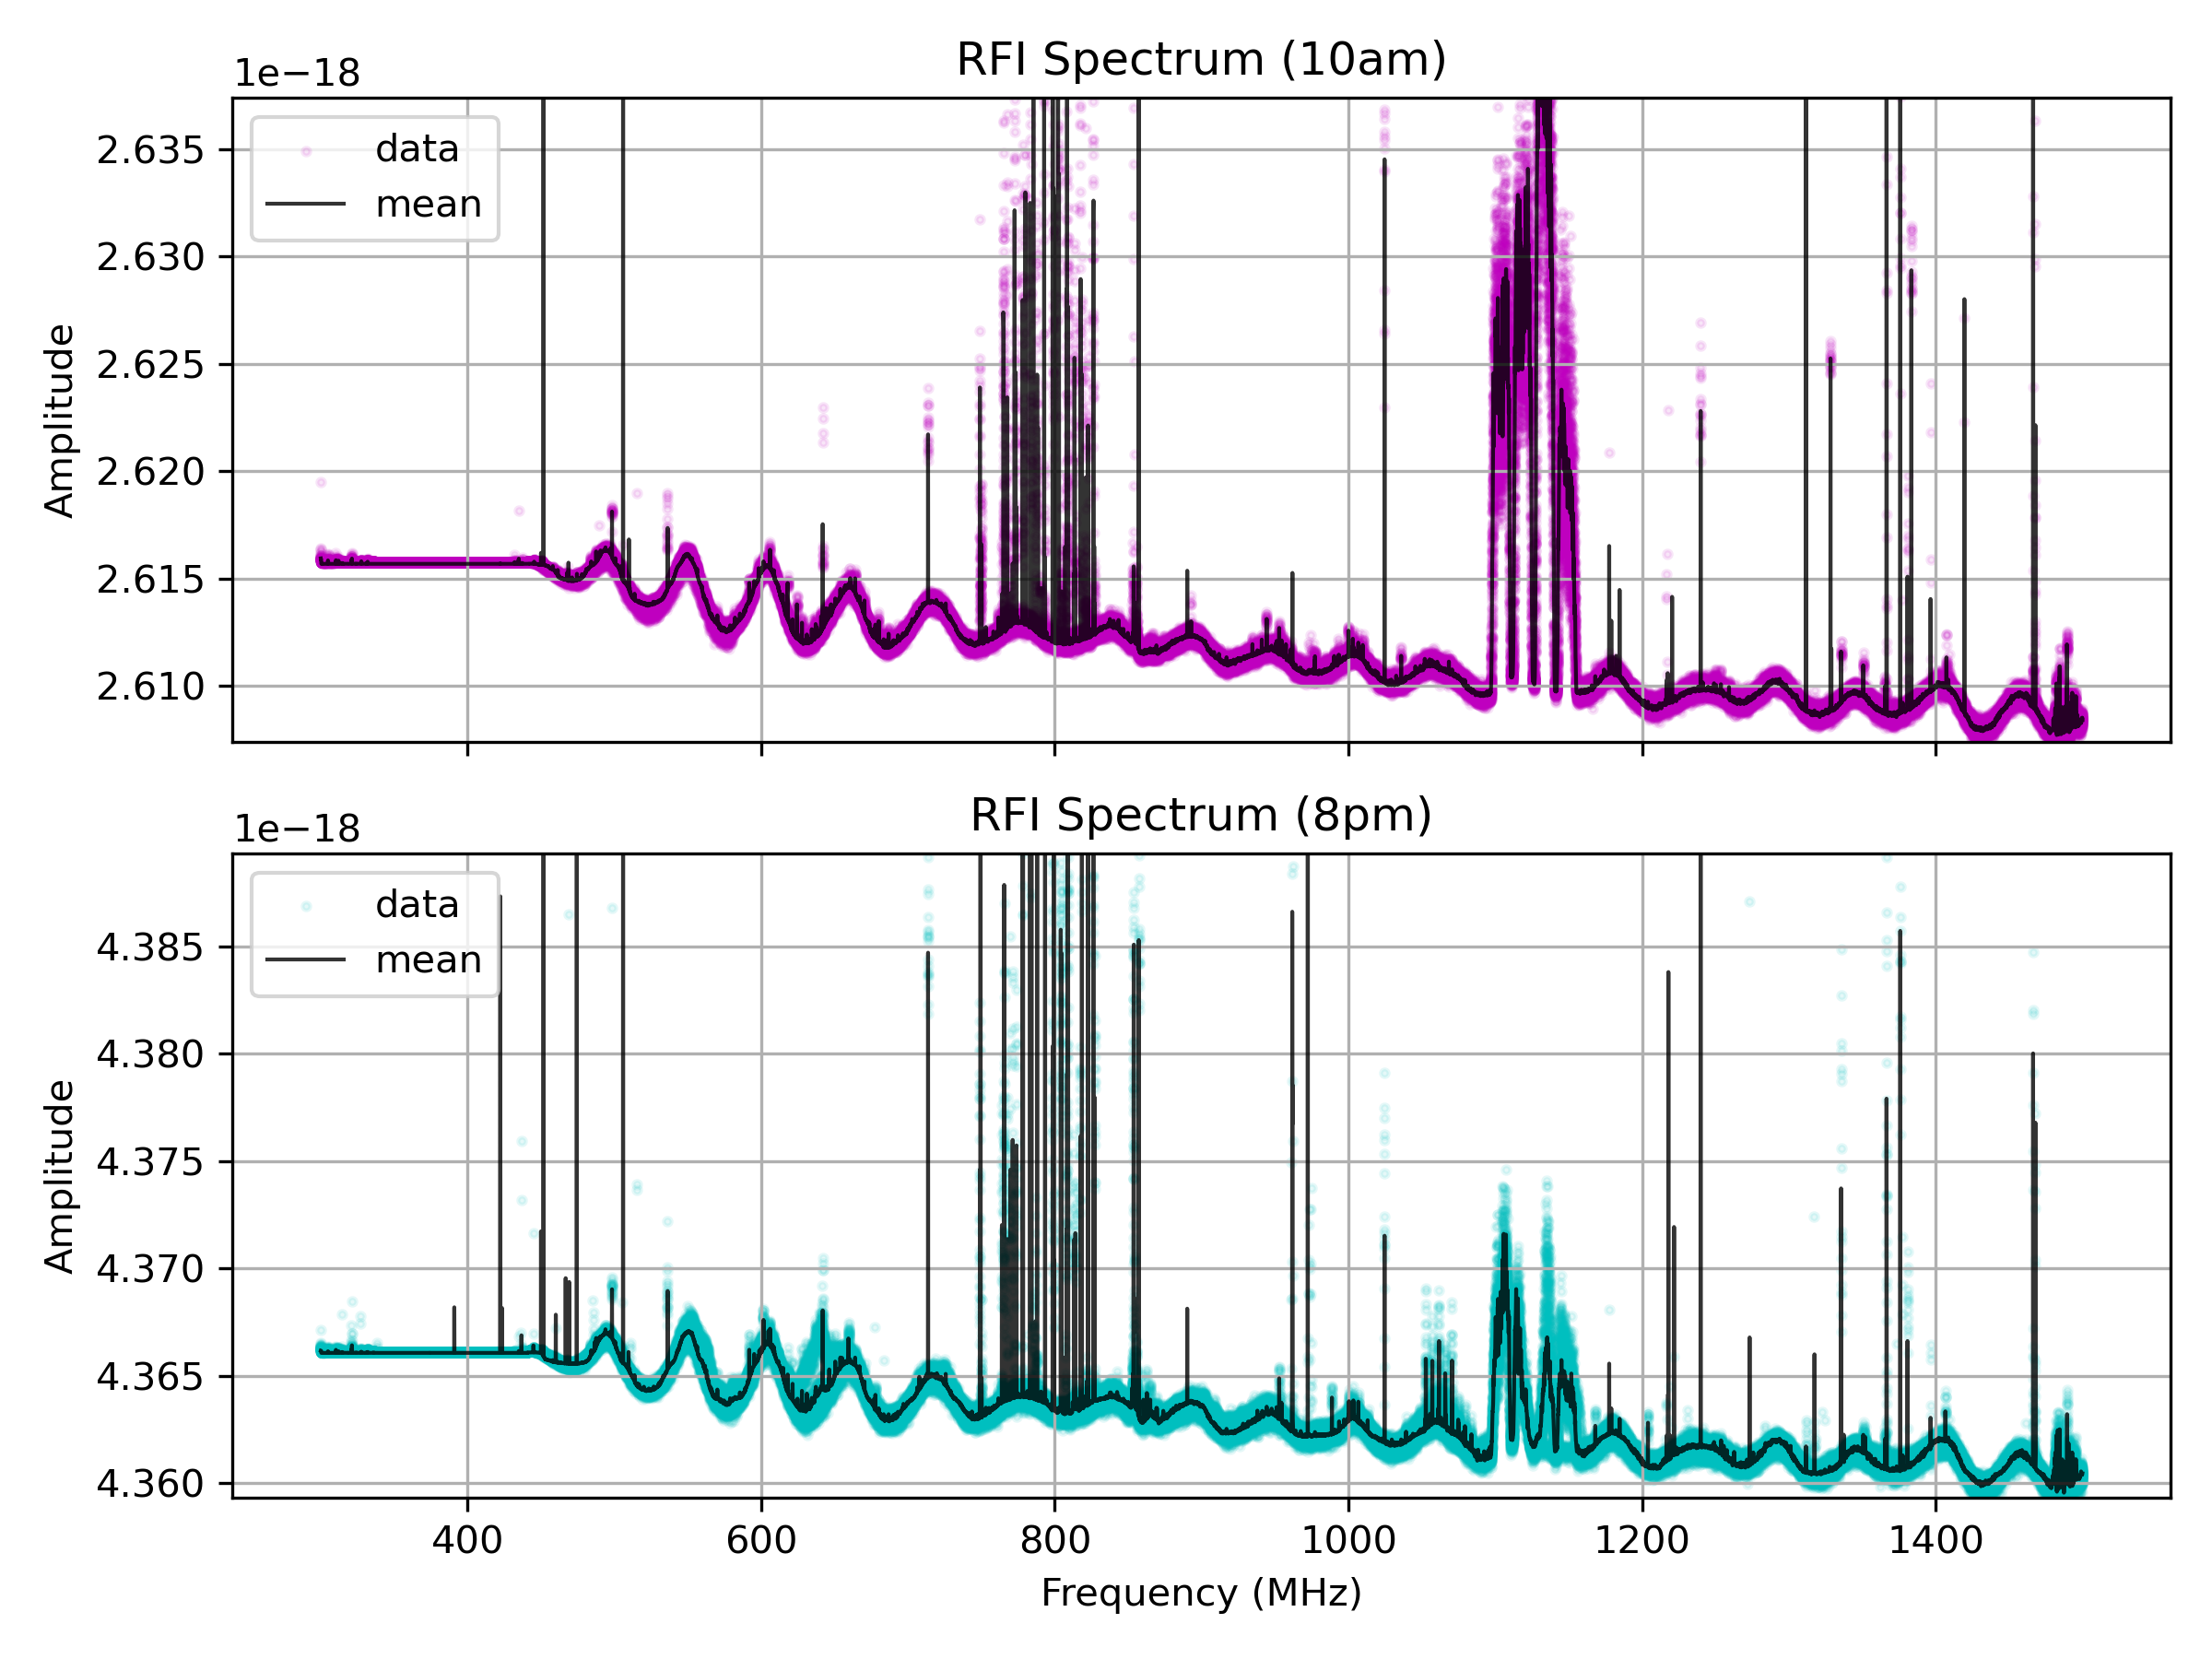
\includegraphics[width=1\linewidth]{thesis/plots/rfi/full_spectrum_overview.png}
    \caption{Enter Caption}
    \label{fig:placeholder}
\end{figure}